\section{Technické vybavení akvária}
    V této kapitole je uveden výčet základní akvaristické techniky nutné k provozu domácího akvária, sekce je rozdělena podle způsobu určení daného vybavení a jejím cílem je seznámit čtenáře blíže s problematikou založení a provozu akvária.
    \subsection{Filtrace vody}
        Úkolem filtru je průběžně odstraňovat z vody nečistoty a to jak mechanické, tak zejména v podobě škodlivých látek vznikajících v akváriu. Filtrační materiál je volen tak, aby tvořil vhodné prostředí pro život filtračních bakterií, které se těmito škodlivými látkami živí \cite{yt-filtrace}. Rozlišujeme tři základní typy akvarijních filtrů -- vnější, vnitřní a závěsné. Na obr.~\ref{fig:filtry-srovnani} se nachází ukázka vybraných zástupců jednotlivých typů.
        
        \textbf{Vnějším filtrem} se rozumí zařízení umístěné obvykle ve skříňce pod akváriem, mívá připojeny dvě hadice -- na vstup a výstup vody. Toto řešení je považováno za nejlepší, protože filtr není omezen rozměry a může tak dosahovat daleko vyššího výkonu a účinnější filtrace díky většímu množství filtračních materiálů. 

        \textbf{Vnitřní filtr} (někdy také ponorný) je levným, ale nepříliš účinným řešením pro malá akvária. Nachází se z velké částo v akváriu a za pomocí motorku tlačí vodu přes obvykle molitanovou náplň.

        \textbf{Závěsný filtr}  je kompromisním řešením.  Cenou i účinností filtrace se pohybuje mezi oběma zmíněnými typy. Nezabírá prostor uvnitř akvária a může tak využít větší objem filtrační hmoty než filtr vnitřní. Instalace je provedena zavěšením na stěnu akvária, je tedy velmi jednoduchá. 

        \begin{figure}[h!]
            \centering
            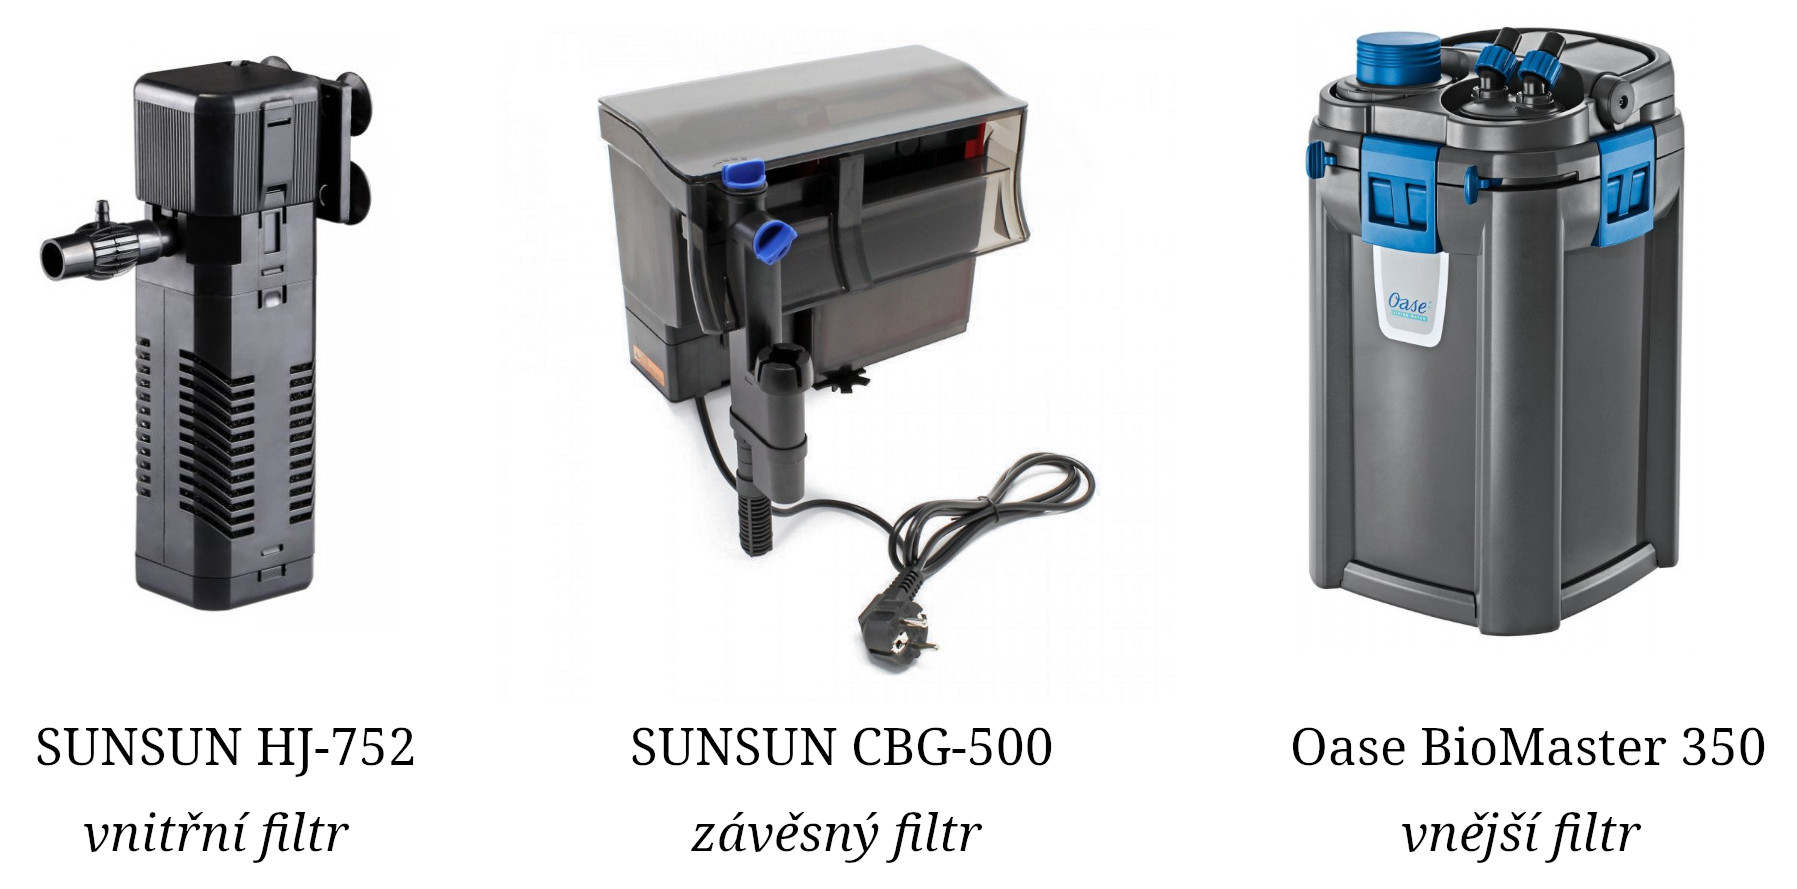
\includegraphics[width=\textwidth]{obrazky/filtry/filtry.jpg}
            \caption{Příklad různých typů filtrů. Fotografie převzaty z \cite{eshop-rostlinna-akvaria}}
            \label{fig:filtry-srovnani}
        \end{figure}

    \subsection{Osvětlení}
        Funkce osvětlení akvária je dvojí. Jednak jde o estetický dojem z pohledu pozorovatele, kdy vhodné nasvícení přidává akváriu na atraktivitě. Druhak se osvětlení snaží nasimulovat osazenstvu akvária přirozené životní podmínky, aby celý ekosystém mohl fungovat.

        Hlavními parametry při výběru svítidla je jeho \textbf{intenzita}, \textbf{spektální charakteristika} a \textbf{spotřeba}. 
        
        Příliš intenzivní světlo zvyšuje riziko nežádoucí tvorby řas a pro ryby může být stresovým faktorem, nízká intenzita zase může způsobit špatný růst rostlin. Na internetu existuje mnoho návodů a tipů na stanovení správné intenzity, ale protože zde hraje roli spousta dalších parametrů jako např. výška hladiny nebo konkrétní typ rostlin, je vhodné tyto hodnoty brát pouze jako orientační a intenzitu osvětlení upravit během provozu podle potřeby. Výpočet se také liší pro jednotlivé typy svítidel. 

        Spektrum světla hraje roli hned z několika důvodů. Rostliny pro tvorbu chlorofylu a následnou fotosyntézu potřebují světlo zejména vlnových délek \qty{440}{nm} (modrá barva) a \qty{660}{nm} (červená barva)~\cite{eshop-ledsolution-svetlo}, pokud by zvolené osvětlení tyto vlnové délky neobsahovalo, nemohou rostliny správně fungovat. Akvárium osvětlené pouze těmito dvěma barvami by ale nevypadalo vizuálně dobře, proto se využívá také širokospektrální bílé světlo, které svým spektrem odpovídá co nejlépe dennímu světlu. 
        Specializovaná svítidla pak nabízejí možnost napodobit světelné spektrum různých vodních prostředí a přizpůsobit se tak i rostlinám a živočichům žijícím ve velkých hloubkách. 

        \begin{figure}[h!]
            \centering
            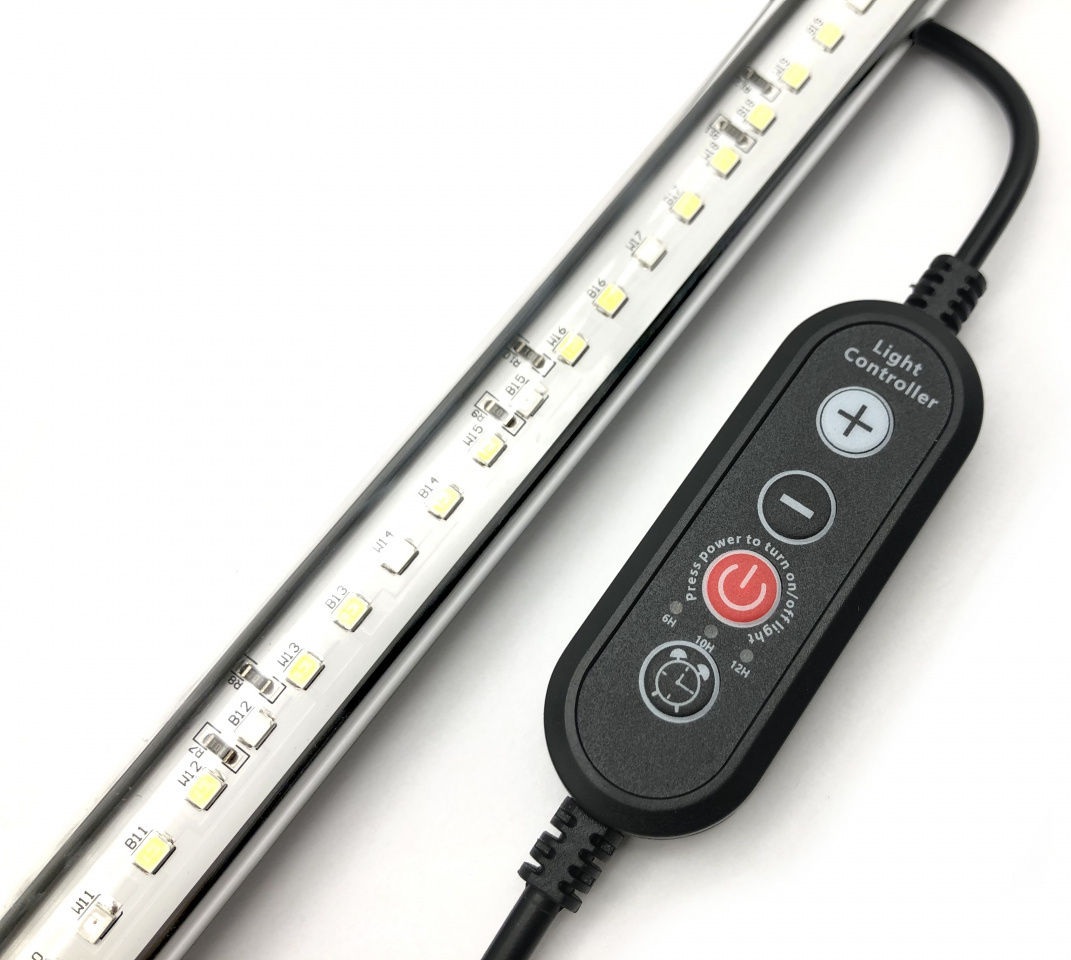
\includegraphics[width=0.6\textwidth]{obrazky/osvetleni/stmivac.jpg}
            \caption{Trubice s LED páskem a manuální stmívač a časovač. Převzato z \cite{eshop-rostlinna-akvaria}.}
            \label{fig:obrazky-osvetleni-stmivac-jpg}
        \end{figure}

        Na trhu jsou v současné době tři typy akvaristických světel: \textbf{zářivky}, \textbf{výbojky}  a \textbf{LED svítidla}~\cite{eshop-rostlinna-akvaria-svetlo}. Zářivky jsou považovány za dnes již nepříliš moderní řešení a bývají nahrazovány LED svítidly, ty se vyznačují lepší účinností (tedy nižší spotřebou), delší životností a širší paletou barev. U zářivek také nebylo možné plynule regulovat intenzitu jako je tomu u LED, skoková změna při zhasnutí světla na noc je pro ryby také zbytečným stresovým faktorem. Co se týče výbojek, ty nacházejí uplatňení zejména pro hluboké nádrže, protože jejich světlo je bodové a intenzita dostačující k prosvícení velkého objemu vody, spotřeba energie je ale v porovnání s LED vysoká, takže pokud to není nezbytně nutné, je lepší se jim vyhnout.   

        Typické domácí akvárium je osvětleno jedním nebo několika samostatně stmivatelnými LED svítidly a to buďto v podobě LED pásků nalepených na hliníkovém profilu anebo hotového svítidla, ve kterém jsou čipy s LED zabudovány napevno. Stmívání je nastavováno buď ručně anebo za pomoci mobilní aplikace dodané výrobcem stmívače. Příklad běžně dostupného výrobku lze vidět na obr.~\ref{fig:obrazky-osvetleni-stmivac-jpg}.

    \subsection{Ohřev}
        Většina okrasných sladkovodních ryb běžně chovaných akvaristy pochází z tropických krajů a vyžaduje teplotu vody v rozmezí 22 -- \qty{26}{\degreeCelsius}~\cite{slavotinek2014}, to je o něco málo vyšší teplota než bývá v domácnosti typická a proto je nutné zajistit akváriu možnost dodatečného ohřevu. Nejčastějsím řešením je ponorné topné těleso na odporové bázi s vlastní termostatovou regulací, viz obr.~\ref{fig:obrazky-topeni-topitko-jpg}.

        \begin{figure}[h!]
            \centering
            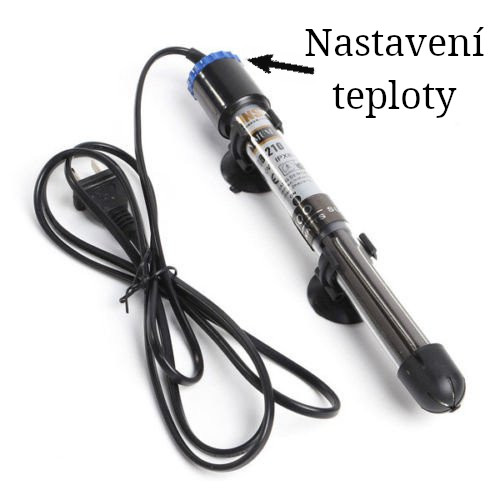
\includegraphics[width=0.7\textwidth]{obrazky/topeni/topitko.jpg}
            \caption{SUNSUN topítko 100W s termostatem. Převzato z \cite{eshop-rostlinna-akvaria}.}
            \label{fig:obrazky-topeni-topitko-jpg}
        \end{figure}
        
        Z principu fungování termostatu vyplývá, že výsledná teplota vody není v čase konstantní, ale osciluje okolo nastavené hodnoty. Rozsah kolísání teploty je pak závislý na hysterezi termostatu, obecně lze říci, že to může být i několik stupňů. Pro většinu aplikací to není velký problém, ale některé druhy ryb mohou být na změny teploty náchylnější, v takovém případě je potřeba buďto vybrat topítko takové, kde výrobce rozsah teplot uvádí a nebo zvolit jiný způsob regulace. 

    \subsection{Monitorování}
        Jak již vyplynulo z úvodních kapitol, v akváriu probíhá celá řada procesů ovlivňujících jeho stav. Klíčem k vytvoření prosperujícího akvária je dosažení rovnováhy a stability mezi nimi za pomoci vhodně nastavené akvarijní techniky. Nejen u začínajících akvaristů se mohou vyskytnout problémy s růstem rostlin, zdravím ryb a nebo třeba výskytem řasy a odhalit příčiny těchto problémů může být mnohdy obtížné, ovzláště pokud není k dispozici dostatečné množství informací o tom, co se v akváriu děje. 
        
        Existuje několik veličin, které úzce souvisí s procesy v akváriu a které je možné také poměrně jednoduše sledovat. Na trhu je celá řada produktů sloužících k tomuto účelu. Většinou je na výběr možnost analogového nebo čistě mechanického přístroje a nebo samostatného digitálního čidla, existují však také komplexní systémy, těm se dále věnuje kapitola  \ref{lab:kapitola-komplexni-reseni}. 

        \subsubsection{Teplota}
            Umístěním teploměru (ať už v analogové nebo digitální podobě) je možné zkontrolovat správné nastavení topného tělesa a následně provést jeho úpravu. Také lze včas získat informaci o jeho případné poruše a nebo třeba jen nedostatečném výkonu. 
        \subsubsection{pH a CO\(\mathbf{_{2}}\)}
            Hodnota pH udává koncentraci 

             
    \subsection{Dostupná komplexní řešení}
    \label{lab:kapitola-komplexni-reseni}
        